\documentclass[10pt]{beamer}

\usetheme{metropolis}
\usepackage{appendixnumberbeamer}

\usepackage{booktabs}
\usepackage[scale=2]{ccicons}
\usepackage{listings}

\definecolor{dkgreen}{rgb}{0,0.6,0}
\definecolor{gray}{rgb}{0.5,0.5,0.5} 
\definecolor{mauve}{rgb}{0.58,0,0.82} 

\lstset{frame=tb,
	language=Java,
	aboveskip=3mm,
	belowskip=3mm,
	showstringspaces=false, 
	columns=flexible,
	basicstyle={\small\ttfamily},
	numbers=none,
	numberstyle=\tiny\color{gray},
	keywordstyle=\color{blue},
	commentstyle=\color{dkgreen},
	stringstyle=\color{mauve},
	breaklines=true,
	breakatwhitespace=true,
	tabsize=3
}

\usepackage{pgfplots}
\usepgfplotslibrary{dateplot}

\usepackage{xspace}
\newcommand{\themename}{\textbf{\textsc{metropolis}}\xspace}

\title{Detecting (Absent) App-to-app Authentication on Cross-device
Short-distance Channels}
%\subtitle{A modern beamer theme}
\date{December 13, 2019}
\author{Stefano Cristalli, Danilo Bruschi, Long Lu, Andrea Lanzi}
\institute{University of Milan Italy Northeastern University Boston US}
\titlegraphic{\hfill
\includegraphics[height=1.5cm]{logo.pdf}}

\begin{document}

\maketitle 

\begin{frame}{Outline}
  \setbeamertemplate{section in toc}[sections numbered]
  \tableofcontents[hideallsubsections]
\end{frame}

\section{Introduction}
\begin{frame}[fragile]{Context}
  \begin{itemize}

  \item Cross-device communications allow nearby devices to directly
    communicate bypassing cellular base stations (BSs) or access
    points (APs) (e.g. {\bf spectral efficiency improvement, energy
      saving, and delay reduction}, etc.)

  \item Without the need for infrastructure, {\bf such a technology
      enables mobile users (e.g., Android) to instantly share
      information (e.g., pictures and videos)}

  \item Such technology is also predominat in {\bf IoT environment}
    where a mobile device is direct connected to the embedded system.

   \end{itemize}


  
\end{frame}

\begin{frame}[fragile]{Current Solutions}
  \begin{itemize}

  \item Several solutions exist for securing cross-device
    communication.  In the Android environment, they allow
    {\bf authentication of devices and communication channels}.

  \item Others solutions {\bf restricts apps’ access to external
      resources, such as Bluetooth, SMS and NFC}, by defining new
    SEAndroid types to represent the resources.

  \item Moroever such {\bf solutions are not able to address several
      communication channels such as: SMS, Audio, Wi-Fi and NFC} due
    to of missing important information for the detection purpose.

  \end{itemize} 

  
\end{frame}

\begin{frame}[fragile]{Contributions}


 \begin{itemize}
  
 %\item This problem is due to the fact that the authentication between
 %  apps is missing. {\bf We name this security issue cross-device
 %    app-to-app communication hijacking, or CATCH}.

 \item We identify a security problem called {\bf cross-device
     app-to-app communication hijacking (CATCH)}, which commonly
   exists in Android apps that use short-distance channels, and
   afflicts all the tested Android version.

 \item We provide a solution to the CATCH problem by {\bf designing
     and developing an authentication scheme detector} that analyzes
   Android apps to discover potential vulnerabilities

 \item {\bf Validate the results of our system on Android apps} with
   manual analysis, and test its resilience in detecting the
   authentication scheme.

\end{itemize}
  
\end{frame}


\section{Cross Device Authentication Scheme}
\begin{frame}[fragile]{Cross-device Authentication Scheme}

  %\begin{itemize}

  %\item Currently, most cross-device, peer-to-peer communications
  %  channels are authenticated by using an {\bf out-of-band scheme}.

  %\end{itemize}
   
  \begin{figure}[bhp]
    \centering
	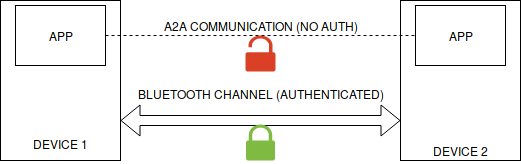
\includegraphics[width=80mm]{img/2-background}
     \end{figure}

     \begin{figure}[bhp]
    \centering
	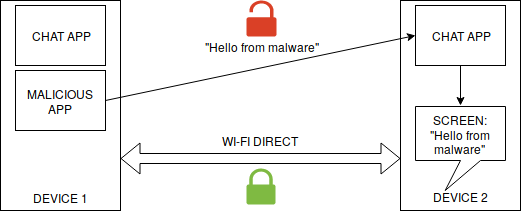
\includegraphics[width=80mm]{img/2-malware}
     \end{figure}
  
 
  
\end{frame}

\begin{frame}[fragile]{Threat Model \& Attack}

  \begin{itemize}


  \item The attacker is able to install a malicious app on the
    mobile's victim phone.

  \item The malicious app can therefore craft custom messages to send
    to the other device, which are displayed as if they were sent from
    the original app.

  \item Depending on the particular context, there are some scenarios
    in which the attack can become very dangerous: {\bf Phishing,
      Malware delivery, Exploitation}.

  \end{itemize}

  
\end{frame}

\section{Approach Overview}
\begin{frame}[fragile]{Challenges}
text.....		
\end{frame}

\begin{frame}[fragile]{Boundary Area: Entry \& Exit Points}
text.....		
\end{frame}

\begin{frame}[fragile]{Detection Strategy}
text.....		
\end{frame}

\section{Technical Details}
\begin{frame}[fragile]{Technical Details}
text.....		
\end{frame}

\section{Experimental Evaluation}
\begin{frame}[fragile]{Experimental Evaluation}
text..... Here we put the experiments that we did		
\end{frame}

\begin{frame}[fragile]{Dataset Composition}
text.....		
\end{frame}

\begin{frame}[fragile]{Results}
text.....		
\end{frame}

\section{Case Studies}
\begin{frame}[fragile]{Data injection on BluetoothChat}
text.....		
\end{frame}

\begin{frame}[fragile]{Data injection on Wi-Fi Direct +}
text.....		
\end{frame}


\section{Discussion}
\begin{frame}[fragile]{Impact \& Limitations}
text.....		
\end{frame}

\section{Conclusion \& Future works}
\begin{frame}[fragile]{Conclusion}
text.....		
\end{frame}

\section*{Thank you for attention}

\section*{Questions?}

\end{document}
